\documentclass[11pt,a4paper]{article}
\usepackage[margin=2.3cm]{geometry}
\usepackage{amsmath,amssymb,bm}
\usepackage{siunitx}
\usepackage{booktabs}
\usepackage{nicefrac}
\usepackage{graphicx}
\usepackage{tikz}
\usetikzlibrary{arrows.meta,calc,positioning,patterns}
\usepackage{pgfplots}
\pgfplotsset{compat=1.17}
\usepackage{enumitem}
\usepackage{float}
\tikzset{capt/.style={text width=5.2cm,align=center}}
\usepackage[colorlinks=true,linkcolor=blue!60!black,urlcolor=blue!60!black]{hyperref}
\usepackage{fancyhdr}
\usepackage{tcolorbox}
\tcbuselibrary{skins,breakable}
\sisetup{per-mode=symbol,detect-all}

\newtcolorbox{keybox}[1]{title={#1},colback=blue!4,colframe=blue!50!black,fonttitle=\bfseries,breakable}
\newtcolorbox{examplebox}[1]{title={#1},colback=green!4,colframe=green!40!black,fonttitle=\bfseries,breakable}
\newtcolorbox{aerobox}[1]{title={#1},colback=orange!5,colframe=orange!60!black,fonttitle=\bfseries,breakable}

\pagestyle{fancy}
\fancyhf{}
\lhead{
\includegraphics[height=0.6cm]{logos/itu_logo_laci.pdf}\ \ UCK 364E Design of Machine Elements}
\setlength{\headheight}{20pt}
\rhead{Lecture 7 -- Notes}
\cfoot{\thepage}

\title{\textbf{UCK 364E Design of Machine Elements}\\[4pt]
\Large Lecture 7: Butt and Fillet Welds\\[2pt]
\large A joint with no fastener, no hole --- and no way to measure whether it is good}
\author{Prof.\ Dr.\ Onur Tunçer\\ Department of Aeronautical Engineering, Istanbul Technical University}
\date{Fall 2026}

\begin{document}
\maketitle

\section*{Learning objectives}
By the end of this lecture you should be able to:
\begin{enumerate}[nosep]
  \item Name the zones of a fusion weld and say what welding does to a hardenable steel and to a
        heat-treated aluminium alloy --- and why the two answers are opposite.
  \item Identify the five joint types and the two weld types, and read and write a weld symbol.
  \item Compute the stress in a butt weld and in a fillet weld, and explain where the factor
        $0.707$ comes from and what the design convention is hiding.
  \item Size a fillet weld for a static load from an allowable stress, and check the parent metal
        beside it.
  \item Apply the reduced allowables that go with a welded 4130 tube and a welded aluminium part,
        and explain what a weld land is for.
  \item Explain why the fatigue strength of an as-welded joint does not rise with the strength of
        the steel, and why it is written in stress \emph{range}.
  \item Use a detail category to predict the life of a welded detail, and rank the common details.
  \item List the weld defects, the inspection method that finds each, and say why welding is
        controlled as a \emph{special process}.
  \item Place a weld on a part so that it is not the first thing to crack.
\end{enumerate}

\section{Why this lecture exists}

Lectures 5 and 6 joined parts with fasteners. Every one of those joints had a hole, and the hole
set the strength: net section, bearing, the stress concentration at the edge. A weld has no hole.
It can develop the full section of the member, it is light, it is leak-tight, and it is cheap.
On paper it is the perfect joint.

\medskip
It is not used to hold an airliner together, and the reasons are the subject of this lecture.

\begin{enumerate}[leftmargin=*,itemsep=2pt]
\item \textbf{A weld changes the material.} You specified an alloy and a temper. In a band a few
  millimetres wide beside every weld, you no longer have it.
\item \textbf{A weld creates its own notch.} The toe of a weld is a sharp change of section with a
  small crack-like flaw already in it. In fatigue, that toe --- not the alloy --- sets the life.
\item \textbf{A weld is continuous.} A crack in a riveted skin stops at the next seam. A crack in a
  welded structure has an unbroken path. The wartime Liberty ships, the first large all-welded
  hulls, taught this the expensive way.
\item \textbf{A weld cannot be verified by measurement.} You can gauge a hole and check a torque.
  Whether a weld is fused at its root cannot be read off the finished part. Its quality has to be
  built in by controlling the process and the welder.
\end{enumerate}

So welding in aerospace lives where its advantages are decisive and its problems can be managed:
steel-tube trusses and engine mounts, landing-gear and engine components that are heat treated
after welding, exhaust systems, pressure vessels and propellant tanks. Project 1 is one of these.

\begin{keybox}{The one idea to carry through the lecture}
For a bolted joint you asked: \emph{how strong is the fastener, and how strong is the plate?} For a
welded joint you must ask three things: how strong is the \emph{weld metal}, how strong is the
\emph{parent metal beside it now}, and --- if the load varies --- \emph{what shape is the toe}.
\end{keybox}

\section{What welding does to the metal}
\label{sec:metal}

\begin{figure}[H]\centering
\resizebox{0.95\textwidth}{!}{% A fusion weld in section, and what happens to hardness across it.
\begin{tikzpicture}[>=Latex,line join=round]
\tikzset{lab/.style={font=\footnotesize}, sm/.style={font=\scriptsize}}
% ---- section ----
\fill[black!8] (-7,0) rectangle (7,1.2);
\fill[black!24] (-0.35,0) -- (-1.25,1.2) -- (-2.45,1.2) -- (-1.55,0) -- cycle;
\fill[black!24] (0.35,0) -- (1.25,1.2) -- (2.45,1.2) -- (1.55,0) -- cycle;
\fill[black!55] (-0.35,0) -- (-1.25,1.2) .. controls (-0.6,1.48) and (0.6,1.48) .. (1.25,1.2) -- (0.35,0) .. controls (0.15,-0.12) and (-0.15,-0.12) .. cycle; % weld metal
\draw[line width=0.7pt] (-7,0) -- (-0.35,0) .. controls (-0.15,-0.12) and (0.15,-0.12) .. (0.35,0) -- (7,0) (-7,1.2) -- (-1.25,1.2) .. controls (-0.6,1.48) and (0.6,1.48) .. (1.25,1.2) -- (7,1.2);
\draw[line width=0.7pt] (-7,0) -- (-7,1.2) (7,0) -- (7,1.2);
\draw[black!70,line width=0.4pt] (-0.35,0) -- (-1.25,1.2) (0.35,0) -- (1.25,1.2);
\node[lab,text=white] at (0,0.65) {weld};
\node[lab] at (-4.6,0.6) {parent metal, unaffected}; \node[lab] at (4.6,0.6) {parent metal, unaffected};
\draw[<-,line width=0.4pt] (-1.85,0.9) -- (-2.6,1.75); \node[lab,anchor=south] at (-3.1,1.72) {heat-affected zone (HAZ)};
\draw[<-,line width=0.4pt] (1.25,1.22) -- (2.3,1.75); \node[lab,anchor=south west] at (2.1,1.72) {toe};
\draw[<-,line width=0.4pt] (0,-0.1) -- (0.9,-0.55); \node[lab,anchor=west] at (0.9,-0.6) {root};
\draw[<-,line width=0.4pt] (0,1.42) -- (0,1.95); \node[lab,anchor=south] at (0,1.92) {reinforcement};
% ---- hardness traverse ----
\begin{scope}[yshift=-4.6cm]
\draw[->] (-7,0) -- (7.3,0) node[lab,anchor=north east] {distance across the weld};
\draw[->] (-7,0) -- (-7,3.5) node[lab,anchor=south west,xshift=-2pt] {hardness (strength)};
\foreach \x in {-2.45,-0.8,0.8,2.45}{\draw[black!45,dashed,line width=0.3pt] (\x,0) -- (\x,3.3);}
\node[sm,black!60] at (-1.8,3.25) {HAZ}; \node[sm,black!60] at (1.8,3.25) {HAZ}; \node[sm,black!60] at (0,3.25) {weld};
% steel: hard HAZ
\draw[line width=1.3pt] plot[smooth,tension=0.55] coordinates {(-7,1.55) (-3.2,1.55) (-2.6,1.7) (-1.9,2.75) (-1.2,2.65) (-0.6,1.95) (0,1.85) (0.6,1.95) (1.2,2.65) (1.9,2.75) (2.6,1.7) (3.2,1.55) (7,1.55)};
\node[lab,anchor=west] at (2.75,2.7) {hardenable steel (4130): \textbf{hard, brittle HAZ}};
% aluminium: soft HAZ
\draw[line width=1.3pt,dash pattern=on 5pt off 2.5pt] plot[smooth,tension=0.55] coordinates {(-7,1.25) (-3.4,1.25) (-2.7,1.1) (-1.9,0.55) (-1.1,0.5) (-0.5,0.62) (0,0.66) (0.5,0.62) (1.1,0.5) (1.9,0.55) (2.7,1.1) (3.4,1.25) (7,1.25)};
\node[lab,anchor=west] at (2.75,0.45) {heat-treated aluminium (6061-T6): \textbf{soft HAZ}};
\end{scope}
\end{tikzpicture}
}
\caption{A fusion weld in section, and the hardness across it. The parent metal next to the weld
has been through a heat treatment nobody specified.}
\label{fig:zones}
\end{figure}

A fusion weld has three regions. The \textbf{weld metal} was liquid: it is a casting, made of
filler and melted parent metal, with a cast structure. The \textbf{heat-affected zone (HAZ)} never
melted but was taken close to melting and cooled quickly by the cold metal around it. Beyond that
the \textbf{parent metal} is as you bought it. The two ends of the weld surface are the
\textbf{toes}; the bottom of the joint is the \textbf{root}.

\medskip
What the HAZ becomes depends entirely on how the alloy gets its strength, and the two alloys that
matter to us go in opposite directions.

\begin{itemize}[leftmargin=*,itemsep=3pt]
\item \textbf{Hardenable steel (4130, 4340).} The HAZ is heated above the transformation
  temperature and then quenched by the surrounding metal. It comes out \emph{harder and more
  brittle} than the parent --- untempered martensite --- and prone to cracking, especially with
  hydrogen present. The cure is to control the cooling (preheat, slow cool), and for a
  heat-treated part to weld first and \emph{then} heat treat the whole assembly.
\item \textbf{Heat-treated aluminium (6061-T6, and every 2xxx and 7xxx alloy).} The temper is a
  fine precipitate that took hours in a furnace to grow. The welding heat dissolves or coarsens it
  in seconds. The HAZ comes out \emph{softer}: 6061-T6, about \SI{290}{MPa} as bought, is worth
  about \SI{165}{MPa} across a weld. Unless the part is solution treated and aged again after
  welding, the strength you paid for is gone locally.
\end{itemize}

\begin{aerobox}{Why airframes are riveted and rockets are welded}
The high-strength airframe alloys, 2024 and 7075, are not fusion weldable in practice: they crack
as the weld freezes, and what survives has lost its temper. That, more than tradition, is why
Lecture 6 spent so long on rivets.

\medskip
A propellant tank is different. It must be leak-tight, it is nearly all membrane, and its alloy can
be chosen for weldability (2219, 2195). The weld is made on a locally thickened strip --- a
\textbf{weld land} --- sized so that the softened metal at the weld is no more highly loaded than
the full-strength skin beside it. And since the 1990s \textbf{friction stir welding} has joined
these alloys without melting them at all: a rotating tool stirs the two edges together in the solid
state. It is how the tanks of current launch vehicles are made, and it is beginning to replace
riveted seams on aircraft.
\end{aerobox}

\subsection*{The processes you will meet}

\begin{center}\footnotesize
\begin{tabular}{@{}p{3.6cm}p{5.2cm}p{6.2cm}@{}}
\toprule
\textbf{Process} & \textbf{Heat source} & \textbf{Where you meet it}\\
\midrule
TIG \ (GTAW, process 141) & arc from a tungsten electrode, inert gas, filler by hand &
  the aerospace standard: tube clusters, thin sheet, engine parts\\[2pt]
MIG / MAG \ (GMAW, 131/135) & arc from a consumable wire, gas shield & general structural work,
  ground equipment\\[2pt]
Manual metal arc \ (SMAW, 111) & coated stick electrode & structural steel; the E60xx--E120xx
  electrodes of Shigley\\[2pt]
Electron beam, laser & a focused beam, deep and narrow & precision engine and gear components,
  very small HAZ\\[2pt]
Resistance spot and seam & current through clamped sheets & sheet-metal assemblies, lightly
  loaded\\[2pt]
Friction stir \ (FSW) & none: mechanical stirring, solid state & aluminium tanks and panels\\
\bottomrule
\end{tabular}
\end{center}

\section{Joints, welds, and the symbol}

\begin{figure}[H]\centering
\resizebox{0.9\textwidth}{!}{% The five joint types, and the two weld types that make them.
\begin{tikzpicture}[line join=round]
\tikzset{pl/.style={fill=black!10,draw=black,line width=0.6pt}, wd/.style={fill=black!70,draw=black,line width=0.4pt},
  ttl/.style={font=\footnotesize\bfseries,anchor=north}, sub/.style={font=\scriptsize,anchor=north,text=black!65,align=center}}
% butt
\begin{scope}
 \path[pl] (-1.5,0) rectangle (-0.08,0.45); \path[pl] (0.08,0) rectangle (1.5,0.45);
 \path[wd] (-0.08,0) -- (-0.32,0.45) .. controls (-0.1,0.6) and (0.1,0.6) .. (0.32,0.45) -- (0.08,0) -- cycle;
 \node[ttl] at (0,-0.75) {Butt}; \node[sub] at (0,-1.15) {groove weld};
\end{scope}
% T
\begin{scope}[xshift=3.6cm]
 \path[pl] (-1.3,0) rectangle (1.3,0.4); \path[pl] (-0.2,0.4) rectangle (0.2,1.7);
 \path[wd] (-0.2,0.4) -- (-0.62,0.4) -- (-0.2,0.82) -- cycle; \path[wd] (0.2,0.4) -- (0.62,0.4) -- (0.2,0.82) -- cycle;
 \node[ttl] at (0,-0.75) {T}; \node[sub] at (0,-1.15) {fillet welds};
\end{scope}
% lap
\begin{scope}[xshift=7.2cm]
 \path[pl] (-1.5,0) rectangle (0.5,0.4); \path[pl] (-0.5,0.4) rectangle (1.5,0.8);
 \path[wd] (-0.5,0.4) -- (-0.92,0.4) -- (-0.5,0.8) -- cycle; \path[wd] (0.5,0.4) -- (0.92,0.4) -- (0.5,0) -- cycle;
 \node[ttl] at (0,-0.75) {Lap}; \node[sub] at (0,-1.15) {fillet welds};
\end{scope}
% corner
\begin{scope}[xshift=10.6cm]
 \path[pl] (-1.2,0) rectangle (0.5,0.4); \path[pl] (0.1,0.4) rectangle (0.5,1.7);
 \path[wd] (0.1,0.4) -- (-0.32,0.4) -- (0.1,0.82) -- cycle;
 \node[ttl] at (-0.2,-0.75) {Corner}; \node[sub] at (-0.2,-1.15) {fillet or groove};
\end{scope}
% edge
\begin{scope}[xshift=13.4cm]
 \path[pl] (-0.42,0) rectangle (-0.02,1.5); \path[pl] (0.02,0) rectangle (0.42,1.5);
 \path[wd] (-0.42,1.5) .. controls (-0.3,1.85) and (0.3,1.85) .. (0.42,1.5) -- cycle;
 \node[ttl] at (0,-0.75) {Edge}; \node[sub] at (0,-1.15) {thin sheet};
\end{scope}
\end{tikzpicture}
}
\caption{Five joint types. They are made with only two kinds of weld: the \emph{groove} (butt)
weld, which fills the gap between two edges, and the \emph{fillet}, which sits in a corner.}
\label{fig:types}
\end{figure}

The distinction that matters for analysis is between the two weld types, not the five joint types.

\begin{itemize}[leftmargin=*,itemsep=2pt]
\item A \textbf{groove weld}, made with full penetration, replaces the section. The load flows
  straight through it. This is the weld you want.
\item A \textbf{fillet weld} joins two surfaces at an angle without preparing the edges. The load
  has to turn a corner to get through it, the unfused root is a built-in crack, and its strength
  is the strength of a small triangle of weld metal. This is the weld you can afford.
\end{itemize}

\subsection*{The weld symbol}

A weld is specified on a drawing by a symbol, not by drawing the bead. Project 1 requires it.

\begin{figure}[H]\centering
\resizebox{0.92\textwidth}{!}{% Anatomy of a weld symbol (ISO 2553), with the joint it describes.
\begin{tikzpicture}[>=Latex,line join=round]
\tikzset{lab/.style={font=\footnotesize}, sm/.style={font=\scriptsize,text=black!70}, pl/.style={fill=black!10,draw=black,line width=0.6pt}}
% ---- the joint ----
\path[pl] (-6.2,-0.4) rectangle (-2.6,0); \path[pl] (-4.6,0) rectangle (-4.2,1.9);
\fill[black!70] (-4.2,0) -- (-3.72,0) -- (-4.2,0.48) -- cycle;
\node[sm,anchor=north] at (-4.4,-0.5) {the joint};
% ---- the symbol ----
\draw[line width=0.8pt,->] (0.2,1.5) -- (-1.0,1.5) -- (-3.95,0.26);
\draw[line width=0.8pt] (0.2,1.5) -- (6.6,1.5) -- (7.2,2.0) (6.6,1.5) -- (7.2,1.0);
\draw[line width=0.5pt,dashed] (0.2,1.28) -- (6.6,1.28);
\draw[line width=0.8pt] (2.3,1.5) -- (2.3,2.15) -- (2.95,1.5);            % fillet symbol on the arrow side
\node[font=\small] at (1.55,1.86) {a5}; \node[font=\small] at (4.3,1.86) {6 $\times$ 40 (60)}; \node[font=\small] at (7.75,1.5) {141};
\draw[line width=0.8pt] (0.2,1.5) circle[radius=0.17];                    % weld all round
\draw[line width=0.8pt] (0.2,1.67) -- (0.2,2.55); \fill (0.2,2.55) -- (0.75,2.38) -- (0.2,2.21) -- cycle; % site weld
% ---- callouts ----
\draw[<-,line width=0.3pt] (-2.4,0.95) -- (-2.6,2.2); \node[sm,anchor=south] at (-2.6,2.2) {arrow: points at the joint};
\draw[<-,line width=0.3pt] (1.55,2.08) -- (1.55,3.0); \node[sm,anchor=south,align=center] at (1.55,3.0) {size: throat $a=\SI{5}{mm}$\\ ($z5$ would be a \SI{5}{mm} leg)};
\draw[<-,line width=0.3pt] (2.55,2.0) -- (3.2,3.9); \node[sm,anchor=south,align=center] at (3.6,3.9) {weld type: fillet};
\draw[<-,line width=0.3pt] (4.3,2.08) -- (5.2,3.0); \node[sm,anchor=south,align=center] at (5.6,3.0) {6 lengths of \SI{40}{mm},\\ gaps of \SI{60}{mm}};
\draw[<-,line width=0.3pt] (7.75,1.72) -- (7.9,2.7); \node[sm,anchor=south,align=center] at (7.9,2.7) {tail: process\\ (141 = TIG)};
\draw[<-,line width=0.3pt] (0.2,1.3) -- (-0.3,0.45); \node[sm,anchor=north,align=center] at (-0.5,0.45) {circle: weld\\ all round};
\draw[<-,line width=0.3pt] (0.5,2.38) -- (-0.4,3.0); \node[sm,anchor=south east,align=right] at (-0.3,2.95) {flag: made on site};
\draw[<-,line width=0.3pt] (4.6,1.26) -- (4.8,0.45); \node[sm,anchor=north,align=center] at (4.9,0.45) {symbol on the solid line: weld on the \emph{arrow} side\\ on the dashed line: the \emph{other} side};
\end{tikzpicture}
}
\caption{The weld symbol of ISO 2553. The American system (AWS A2.4) uses the same skeleton but
gives the fillet size as the \emph{leg}, and has no dashed line: below the reference line means
arrow side, above means other side.}
\label{fig:symbol}
\end{figure}

\begin{keybox}{Throat or leg --- say which}
A fillet is sized by its throat $a$ or by its leg $z$, and $a=0.707\,z$. A ``5 mm fillet'' is
therefore two different welds, one with twice the cross-section of weld metal of the other. ISO
drawings write \textbf{a5} or \textbf{z7}; write the letter. Shigley and American practice use the
leg, and call it $h$. These notes use $h$ for the leg and $a$ for the throat throughout.
\end{keybox}

\section{Butt welds}

For a full-penetration butt weld in a plate of thickness $t$ and width $l$, carrying a tensile
force $F$ or a shear force $V$,
\begin{equation}
\sigma=\frac{F}{t\,l},\qquad\qquad \tau=\frac{V}{t\,l}.
\end{equation}
The throat is the plate thickness. \textbf{The reinforcement does not count}: the bulge of weld
metal above the surface adds no strength, because the plate beside it is still only $t$ thick. What
it does add is a toe. For static loading it is harmless; for fatigue it is the problem, and the
best butt welds are ground flush (\S\ref{sec:fatigue}).

\medskip
A butt weld made from one side without full penetration is a different object. The unfused root is
a crack perpendicular to the load, the throat is less than $t$, and the load path is eccentric.
Partial-penetration butt welds are not used in tension in anything that matters.

\section{Fillet welds}
\label{sec:fillet}

\begin{figure}[H]\centering
\resizebox{0.95\textwidth}{!}{% Fillet weld: the names, and the throat plane of a transverse fillet.
\begin{tikzpicture}[>=Latex,line join=round]
\tikzset{pl/.style={fill=black!10,draw=black,line width=0.7pt}, lab/.style={font=\footnotesize}, dimn/.style={<->,black!70,line width=0.4pt}}
% ---------- geometry ----------
\path[pl] (-3.4,-0.8) rectangle (3.0,0); \path[pl] (-0.9,0) rectangle (0,3.3);
\fill[black!55] (0,0) -- (2.2,0) -- (0,2.2) -- cycle; \draw[line width=0.7pt] (0,0) -- (2.2,0) -- (0,2.2) -- cycle;
\draw[white,line width=1.1pt] (0,0) -- (1.1,1.1);
\draw[dimn] (0,-1.15) -- (2.2,-1.15); \draw[black!60,line width=0.3pt] (2.2,-0.85) -- (2.2,-1.3) (0,-0.85) -- (0,-1.3);
\node[lab,anchor=north] at (1.1,-1.18) {leg $h$ \ (ISO: $z$)};
\draw[dimn] (-1.25,0) -- (-1.25,2.2); \draw[black!60,line width=0.3pt] (-0.95,2.2) -- (-1.4,2.2); \node[lab,anchor=east] at (-1.3,1.1) {$h$};
\draw[<-,line width=0.4pt] (0.62,0.62) -- (2.3,2.0); \node[lab,anchor=west,align=left] at (2.3,2.15) {throat\\ $a=0.707\,h$};
\draw[<-,line width=0.4pt] (2.2,0.03) -- (3.2,0.8); \node[lab,anchor=west] at (3.2,0.85) {toe};
\draw[<-,line width=0.4pt] (0.03,2.2) -- (0.9,3.0); \node[lab,anchor=west] at (0.9,3.05) {toe};
\draw[<-,line width=0.4pt] (0.06,0.06) -- (-1.9,0.9); \node[lab,anchor=east] at (-1.9,0.95) {root};
\draw[<-,line width=0.4pt] (1.5,0.72) -- (2.4,1.1); \node[lab,anchor=west] at (2.4,1.15) {face};
% ---------- throat plane at angle theta ----------
\begin{scope}[xshift=8.6cm]
\path[pl] (-0.9,0) rectangle (0,3.3); \path[pl] (-3.0,-0.8) rectangle (3.4,0);
\draw[line width=0.7pt,fill=black!25] (0,0) -- (2.2,0) -- (0,2.2) -- cycle;
% cut plane through the root at theta from the vertical leg
\draw[line width=1.2pt] (0,0) -- (0.84,1.36);
\draw[line width=0.4pt] (0,0.75) arc[start angle=90,end angle=58.3,radius=0.75]; \node[lab] at (0.27,1.02) {$\theta$};
\draw[->,line width=1.1pt] (-2.6,1.7) -- (-1.0,1.7); \node[lab,anchor=south] at (-1.8,1.72) {$F$};
\draw[->,line width=1.1pt] (0.42,0.68) -- ++(-31.7:1.25);
\draw[->,line width=1.1pt] (0.42,0.68) -- ++(58.3:1.25);
\node[lab,anchor=south west] at (1.1,1.66) {$F_s=F\sin\theta$};
\node[lab,anchor=west] at (1.55,0.3) {$F_n=F\cos\theta$};
\node[lab,anchor=west,align=left] at (0.6,3.0) {plane length\\ $h/(\sin\theta+\cos\theta)$};
\draw[<-,line width=0.4pt] (0.7,1.18) -- (1.1,2.6);
\end{scope}
\end{tikzpicture}
}
\caption{Left: the names. The throat is the shortest distance from the root to the face, and for
an equal-leg fillet it is $0.707h$. Right: a transverse fillet cut on a plane through the root at
an angle $\theta$.}
\label{fig:fillet}
\end{figure}

\subsection{The stress on the throat}

Take a transverse fillet of leg $h$ and length $l$ carrying a force $F$, and cut it on a plane
through the root at angle $\theta$ (figure~\ref{fig:fillet}, right). The plane has length
$h/(\sin\theta+\cos\theta)$, and the force resolves into a shear $F_s=F\sin\theta$ and a normal
force $F_n=F\cos\theta$, so
\begin{equation}
\tau=\frac{F}{h\,l}\,\sin\theta\,(\sin\theta+\cos\theta),\qquad
\sigma=\frac{F}{h\,l}\,\cos\theta\,(\sin\theta+\cos\theta).
\end{equation}
The shear is largest at $\theta=\ang{67.5}$, where $\tau_{\max}=1.207\,F/(hl)$. The von Mises
stress is largest at $\theta=\ang{62.5}$, where $\sigma'=2.16\,F/(hl)$.

\medskip
Nobody designs with those. The real stress field in a fillet is far from uniform --- it peaks at
the root and the toe --- and this free-body analysis is only a model. Design practice uses a
simpler and more conservative one.

\begin{keybox}{The design convention for fillet welds}
\textbf{Whatever the direction of the load, divide the force by the throat area and call the
result a shear stress:}
\begin{equation}
\tau=\frac{F}{0.707\,h\,l}=\frac{1.414\,F}{h\,l}.
\label{eq:fillet}
\end{equation}
For a parallel fillet this is the true average shear on the throat. For a transverse fillet it
overstates the maximum shear by 17 per cent ($1.414$ against $1.207$). It ignores the normal
stress and the stress concentration entirely, and makes up for both through the allowable.
\end{keybox}

\subsection{Parallel and transverse}

\begin{figure}[H]\centering
\resizebox{0.95\textwidth}{!}{% A lap joint seen from above: parallel (longitudinal) and transverse fillets.
\begin{tikzpicture}[>=Latex,line join=round]
\tikzset{lab/.style={font=\Large}}
\begin{scope}
\fill[black!8] (-3.6,-1.5) rectangle (1.2,1.5); \draw[line width=0.6pt] (-3.6,-1.5) rectangle (1.2,1.5);
\fill[black!22] (-1.6,-0.8) rectangle (4.2,0.8); \draw[line width=0.6pt] (-1.6,-0.8) rectangle (4.2,0.8);
\fill[black!75] (-1.6,0.8) rectangle (1.2,0.98); \fill[black!75] (-1.6,-0.8) rectangle (1.2,-0.98);
\draw[->,line width=1.2pt] (4.3,0) -- (5.5,0) node[lab,anchor=west] {$F$};
\draw[->,line width=1.2pt] (-3.7,0) -- (-4.9,0) node[lab,anchor=east] {$F$};
\draw[<->,black!70,line width=0.4pt] (-1.6,1.25) -- (1.2,1.25); \node[lab,anchor=south,fill=black!8,inner sep=1pt] at (-0.2,1.27) {$l$};
\node[lab,anchor=north] at (0.4,-1.7) {\textbf{Parallel fillets}: the weld runs along the load};
\end{scope}
\begin{scope}[xshift=12.6cm]
\fill[black!8] (-3.6,-1.5) rectangle (1.2,1.5); \draw[line width=0.6pt] (-3.6,-1.5) rectangle (1.2,1.5);
\fill[black!22] (-1.6,-0.8) rectangle (4.2,0.8); \draw[line width=0.6pt] (-1.6,-0.8) rectangle (4.2,0.8);
\fill[black!75] (-1.78,-0.8) rectangle (-1.6,0.8);
\draw[->,line width=1.2pt] (4.3,0) -- (5.5,0) node[lab,anchor=west] {$F$};
\draw[->,line width=1.2pt] (-3.7,0) -- (-4.9,0) node[lab,anchor=east] {$F$};
\node[lab,anchor=north] at (0.4,-1.7) {\textbf{Transverse fillet}: the weld runs across the load};
\end{scope}
\end{tikzpicture}
}
\caption{The same lap joint welded two ways.}
\label{fig:loading}
\end{figure}

Tests show a transverse fillet is roughly half as strong again as a parallel one of the same size,
but it deforms much less before it breaks. Two consequences follow. First, the convention of
equation~\eqref{eq:fillet} is safe for both. Second, \emph{a joint with both kinds does not use
them together}: the stiff transverse weld takes the load and breaks before the parallel welds have
stretched enough to help. It is the same lesson as mixing rivets and bolts in Lecture 6.

\medskip
For a parallel fillet the stress is not uniform along the length either. Like the row of fasteners
in Lecture 6, the ends carry more than the middle. A long parallel weld is worth less per
millimetre than a short one, and weld ends are where the cracks start.

\section{Static strength}
\label{sec:static}

\subsection{Weld metal, and matching}

Filler metal is chosen to \emph{match or overmatch} the parent: the weld metal should be at least
as strong as what it joins, so that a properly made butt weld breaks in the plate. For the coated
electrodes of structural steel the number in the name is the minimum tensile strength in ksi.

\begin{center}\footnotesize
\begin{tabular}{@{}lccc@{}}
\toprule
\textbf{Electrode} & $S_{ut}$, MPa & $S_y$, MPa & Elongation, \%\\
\midrule
E60xx & 427 & 345 & 17--25\\
E70xx & 482 & 393 & 22\\
E80xx & 551 & 462 & 19\\
E90xx & 620 & 531 & 14--17\\
E100xx & 689 & 600 & 13--16\\
E120xx & 827 & 737 & 14\\
\bottomrule
\end{tabular}
\hfill
\begin{tabular}{@{}lll@{}}
\toprule
\textbf{Loading} & \textbf{Weld} & \textbf{Allowable}\\
\midrule
Tension & butt & $0.60\,S_y$\\
Bearing & butt & $0.90\,S_y$\\
Bending & butt & $0.60$--$0.66\,S_y$\\
Compression & butt & $0.60\,S_y$\\
Shear & butt or fillet & $0.30\,S_{ut}$ (weld metal)\\
\bottomrule
\end{tabular}
\end{center}

\noindent These are the structural-steel values Shigley tabulates (his Tables 9--3 and 9--4, after
the AISC code). Two things to notice. The shear allowable is on the \emph{weld metal} tensile
strength. And the parent metal beside the weld has to be checked as well: in shear along the leg
it is limited to $0.40\,S_y$ of the parent.

\begin{examplebox}{Example 7.1 --- a bar lap-welded with two parallel fillets}
A $60\times\SI{8}{mm}$ steel bar ($S_y=\SI{355}{MPa}$) is lap-welded to a gusset with two parallel
fillets, each of leg $h=\SI{6}{mm}$ and length $l=\SI{75}{mm}$, using E70xx electrode. What static
load can the joint carry?

\medskip
\textbf{Weld metal.} $\tau_{\text{all}}=0.30\times482=\SI{145}{MPa}$. Throat area
$=2\times0.707\times6\times75=\SI{636}{mm^2}$.
\[ F=145\times636=\SI{92.0}{kN} \]
\textbf{Parent metal in shear along the legs.} $\tau_{\text{all}}=0.40\times355=\SI{142}{MPa}$ on
$2\times6\times75=\SI{900}{mm^2}$: \ $F=\SI{128}{kN}$.

\textbf{The bar itself in tension.} $0.60\times355=\SI{213}{MPa}$ on $60\times8=\SI{480}{mm^2}$:
\ $F=\SI{102}{kN}$.

\medskip
\textbf{The weld governs, at \SI{92}{kN}} --- 90 per cent of what the bar could carry. To develop
the whole bar the welds would need to be $102\,000/(2\times0.707\times6\times145)=\SI{83}{mm}$
long. Eight millimetres of extra weld on each side is the difference between a joint that is the
weak link and one that is not.
\end{examplebox}

\subsection{Aerospace allowables: the parent metal beside the weld}

In structural steel the weld metal usually governs. In aerospace alloys it is usually the other
way round: the question is what is left of the parent.

\begin{aerobox}{Welded 4130 tube --- what Project 1 needs}
Normalised 4130 tube has $F_{tu}\approx\SI{655}{MPa}$ (\SI{95}{ksi}). Welded and \emph{not} heat
treated afterwards --- the normal condition of a tube truss --- the handbook value for the metal
beside the weld is lower, and it depends on the geometry:

\begin{center}\small
\begin{tabular}{@{}ll@{}}
\toprule
Weld at $30^\circ$ or less to the tube axis (scarf, fishmouth) & $F_{tu}=\SI{620}{MPa}$ \ (\SI{90}{ksi})\\
All other welds & $F_{tu}=\SI{552}{MPa}$ \ (\SI{80}{ksi})\\
\bottomrule
\end{tabular}
\end{center}

\noindent These are the long-standing values of MIL-HDBK-5 (section 8.2), quoted here as classroom
figures: take the current MMPDS table for real work. The weld metal itself is separately limited,
to 85 per cent of its minimum tensile strength.

\medskip
Welds are also one of the few joints \emph{exempt} from the fitting factor of 1.15. CS/FAR 25.625
excuses ``joints made under approved practices and based on comprehensive test data'', and names
welded joints. The price of that exemption is the phrase \emph{approved practices}:
\S\ref{sec:process}.
\end{aerobox}

\begin{figure}[H]\centering
\resizebox{0.95\textwidth}{!}{% Three ways to join a 4130 tube end, and why the angle of the weld matters.
\begin{tikzpicture}[line join=round,>=Latex]
\tikzset{tb/.style={fill=black!10,draw=black,line width=0.7pt}, wl/.style={black,line width=2.4pt,line cap=round},
  ttl/.style={font=\normalsize\bfseries,anchor=north}, sub/.style={font=\small,anchor=north,text=black!65,align=center}}
\begin{scope}
 \path[tb] (-2.2,0) rectangle (2.2,0.9); \draw[wl] (0,0) -- (0,0.9);
 \draw[->,line width=0.9pt] (2.3,0.45) -- (3.0,0.45); \draw[->,line width=0.9pt] (-2.3,0.45) -- (-3.0,0.45);
 \node[ttl] at (0,-0.3) {Square butt}; \node[sub] at (0,-0.85) {the whole heat-affected band lies\\ across the load};
\end{scope}
\begin{scope}[xshift=6.6cm]
 \path[tb] (-2.2,0) rectangle (2.2,0.9); \draw[wl] (-0.78,0) -- (0.78,0.9);
 \draw[line width=0.4pt] (-0.78,0) ++(0.9,0) arc[start angle=0,end angle=30,radius=0.9]; \node[font=\scriptsize] at (0.55,0.2) {$30^\circ$};
 \draw[->,line width=0.9pt] (2.3,0.45) -- (3.0,0.45); \draw[->,line width=0.9pt] (-2.3,0.45) -- (-3.0,0.45);
 \node[ttl] at (0,-0.3) {Scarf, $30^\circ$ or less}; \node[sub] at (0,-0.85) {longer weld, and no section\\ is all heat-affected};
\end{scope}
\begin{scope}[xshift=13.2cm]
 \path[tb] (-2.2,0) rectangle (2.2,0.9);
 \draw[wl] (0.9,0.9) -- (-0.6,0.45) -- (0.9,0);
 \draw[->,line width=0.9pt] (2.3,0.45) -- (3.0,0.45); \draw[->,line width=0.9pt] (-2.3,0.45) -- (-3.0,0.45);
 \node[ttl] at (0,-0.3) {Fishmouth}; \node[sub] at (0,-0.85) {the scarf, folded: the usual\\ splice and sleeve end};
\end{scope}
\end{tikzpicture}
}
\caption{Why the angle matters. A square butt puts the whole heat-affected band across the load
path at one station. A scarf or a fishmouth spreads it along the tube.}
\label{fig:tube}
\end{figure}

\begin{examplebox}{Example 7.2 --- a welded 4130 tube in tension}
An engine-mount member is a $25.4\times\SI{0.889}{mm}$ ($1\times0.035$ in) 4130N tube carrying a
limit tensile load of \SI{20}{kN}. Its end is welded to a fitting.

\medskip
Area: $A=\pi(D-t)\,t=\pi(25.4-0.889)(0.889)=\SI{68.5}{mm^2}$. \ Ultimate load: $1.5\times20=
\SI{30}{kN}$ (no fitting factor on the weld).

\begin{center}\small
\begin{tabular}{@{}llll@{}}
\toprule
Section & $F_{tu}$, MPa & Strength, kN & Margin\\
\midrule
Tube, away from the weld & 655 & 44.8 & $+0.49$\\
At a square-cut welded end & 552 & 37.8 & $\mathbf{+0.26}$\\
At a $30^\circ$ fishmouth end & 620 & 42.4 & $+0.41$\\
\bottomrule
\end{tabular}
\end{center}

The weld costs 16 per cent of the tube if it is cut square and 5 per cent if it is fishmouthed. The
margin you report is the one at the weld, not the one in the tube catalogue --- and the choice
between them is made with a hacksaw, before the torch is lit.
\end{examplebox}

\begin{examplebox}{Example 7.3 --- how thick must a weld land be?}
A 6061-T6 panel, \SI{4}{mm} thick, is butt-welded and \emph{not} re-heat-treated. Parent
$F_{tu}=\SI{290}{MPa}$; across the weld $F_{tu}=\SI{165}{MPa}$.

\medskip
Per \SI{50}{mm} of width the plain panel carries $290\times200=\SI{58}{kN}$; at the weld it carries
$165\times200=\SI{33}{kN}$. The joint is worth \textbf{57 per cent} of the panel.

\medskip
To restore the full strength without re-heat-treating, thicken the panel locally so that the
softened zone carries the same load: $t_{\text{land}}=4\times290/165=\SI{7.0}{mm}$. That thickened
strip, a few times the HAZ width, is a weld land. It is why a machined tank panel is thin
everywhere except along its edges.
\end{examplebox}

\section{Fatigue: the toe decides}
\label{sec:fatigue}

Everything in Lectures 2 to 4 assumed you knew the material's endurance limit and corrected it for
surface, size and notches. For a welded joint that approach breaks down, and it is worth being
clear about why.

\begin{figure}[H]\centering
\resizebox{\textwidth}{!}{% Why a weld is a fatigue problem: the toe, and the residual stress.
\begin{tikzpicture}[>=Latex,line join=round]
\tikzset{lab/.style={font=\footnotesize}, sm/.style={font=\scriptsize}}
% ---- (a) the toe ----
\begin{scope}
\fill[black!10] (-3.2,-1.6) rectangle (3.2,0); \draw[line width=0.7pt] (-3.2,-1.6) -- (-3.2,0) (3.2,-1.6) -- (3.2,0);
\fill[black!50] (-0.6,0) .. controls (-0.2,1.5) and (1.6,1.6) .. (3.2,1.45) -- (3.2,0) -- cycle;
\draw[line width=0.7pt] (-3.2,0) -- (-0.74,0) .. controls (-0.66,-0.1) and (-0.58,-0.06) .. (-0.6,0.02) .. controls (-0.2,1.5) and (1.6,1.6) .. (3.2,1.45);
\draw[red!70!black,line width=1.3pt] (-0.66,-0.05) -- (-0.52,-0.42);
\foreach \y/\s in {-0.5/0,-0.9/0,-1.3/0}{\draw[->,black!60,line width=0.5pt] (-3.9,\y) -- (-3.3,\y);}
\draw[black!60,line width=0.5pt] plot[smooth,tension=0.6] coordinates {(-3.2,-0.25) (-1.8,-0.26) (-1.0,-0.2) (-0.72,-0.12) (-0.55,0.25) (-0.2,0.75)};
\draw[black!60,line width=0.5pt] plot[smooth,tension=0.6] coordinates {(-3.2,-0.6) (-1.6,-0.6) (-0.6,-0.5) (0.2,-0.2) (1.2,0.35) (3.2,0.5)};
\draw[black!60,line width=0.5pt] plot[smooth,tension=0.6] coordinates {(-3.2,-1.0) (-1.0,-1.0) (0.6,-0.85) (3.2,-0.7)};
\draw[<-,line width=0.4pt] (-0.72,-0.06) -- (-1.9,1.0); \node[lab,anchor=south,align=center] at (-2.2,1.0) {undercut and a sharp angle:\\ the stress concentrates here};
\draw[<-,line width=0.4pt] (-0.5,-0.36) -- (0.5,-1.15); \node[lab,anchor=west,align=left,text=red!70!black] at (0.5,-1.2) {slag intrusion, 0.1--\SI{0.4}{mm}:\\ \textbf{a crack that is already there}};
\node[lab,anchor=north] at (0,-1.8) {\textbf{(a) The weld toe}};
\end{scope}
% ---- (b) residual stress across a butt weld ----
\begin{scope}[xshift=9.4cm,yshift=-0.55cm]
\fill[black!10] (-3.6,-1.0) rectangle (3.6,-0.7); \fill[black!55] (-0.35,-1.0) rectangle (0.35,-0.7); \draw[line width=0.6pt] (-3.6,-1.0) rectangle (3.6,-0.7);
\draw[->] (-3.8,0.6) -- (3.9,0.6); \draw[->] (0,-0.45) -- (0,2.75);
\draw[line width=1.3pt] plot[smooth,tension=0.6] coordinates {(-3.6,0.42) (-2.4,0.2) (-1.5,0.1) (-0.9,0.6) (-0.45,1.9) (0,2.25) (0.45,1.9) (0.9,0.6) (1.5,0.1) (2.4,0.2) (3.6,0.42)};
\draw[dashed,black!55,line width=0.4pt] (-3.6,2.25) -- (3.6,2.25); \node[sm,anchor=south east] at (3.6,2.25) {$\approx$ yield strength};
\node[sm,anchor=west] at (0.55,1.55) {tension}; \node[sm,anchor=north] at (-1.9,0.08) {compression};
\node[sm,anchor=west] at (3.95,0.6) {};
\node[lab,anchor=north] at (0,-1.25) {\textbf{(b) Residual stress along the weld, as welded}};
\end{scope}
\end{tikzpicture}
}
\caption{The two things that make an as-welded joint a fatigue problem. (a) The toe is a notch
with a flaw in it. (b) The weld is left stretched: residual tension close to yield along the weld,
balanced by compression further out.}
\label{fig:toe}
\end{figure}

\begin{enumerate}[leftmargin=*,itemsep=3pt]
\item \textbf{There is no initiation phase.} The toe of an arc weld carries small sharp intrusions,
  typically a few tenths of a millimetre deep. Lecture 3 called that an initial crack. The life of
  a welded detail is almost entirely \emph{crack growth} from the first cycle --- which is why
  welded S--N curves have a slope of 3, the Paris exponent of steel.
\item \textbf{Stronger steel does not help.} Crack growth rate hardly depends on the strength of a
  steel. So an as-welded joint in a \SI{700}{MPa} steel has the same fatigue life as the same joint
  in a \SI{350}{MPa} steel. You pay for the strength and the weld gives none of it back.
\item \textbf{The mean stress is already at yield.} With residual tension near yield at the toe,
  every cycle runs from about yield downward, whatever the applied mean. The applied mean stress
  stops mattering. Welded fatigue data is therefore written in \textbf{stress range}
  $\Delta\sigma$, with no Goodman correction.
\end{enumerate}

\subsection{Detail categories}

Because the life depends on the geometry of the detail and not on the alloy, welded joints are
\emph{classified}. Each standard detail has a category, and the category is a number: the stress
range, in MPa, that the detail survives for $2\times10^{6}$ cycles. The International Institute of
Welding calls it the FAT class.
\begin{equation}
\boxed{\;N=2\times10^{6}\left(\frac{\mathrm{FAT}}{\Delta\sigma}\right)^{3}\;}
\label{eq:fat}
\end{equation}
down to a knee at $10^{7}$ cycles. $\Delta\sigma$ is the \emph{nominal} stress range in the member
at the detail: the stress concentration of the weld is already inside the category.

\begin{figure}[H]\centering
\resizebox{0.86\textwidth}{!}{% S-N curves for classified welded details (IIW, steel): stress range against cycles.
\begin{tikzpicture}
\begin{loglogaxis}[width=13.4cm,height=8.2cm,xmin=1e4,xmax=1e8,ymin=10,ymax=1000,
  xlabel={Cycles to failure, $N$},ylabel={Stress range $\Delta\sigma$, MPa},
  label style={font=\footnotesize},tick label style={font=\footnotesize},grid=both,
  major grid style={black!22},minor grid style={black!8},clip=true]
% FAT lines: N = 2e6 (FAT/ds)^3 down to the knee at 1e7, then flat
\addplot[black,line width=1.1pt,domain=1e4:1e7,samples=2] {160*(2e6/x)^(1/3)};
\addplot[black,line width=0.7pt,dashed,domain=1e7:1e8,samples=2] {93.57};
\addplot[black,line width=1.1pt,domain=1e4:1e7,samples=2] {112*(2e6/x)^(1/3)};
\addplot[black,line width=0.7pt,dashed,domain=1e7:1e8,samples=2] {65.50};
\addplot[black,line width=1.1pt,domain=1e4:1e7,samples=2] {80*(2e6/x)^(1/3)};
\addplot[black,line width=0.7pt,dashed,domain=1e7:1e8,samples=2] {46.78};
\addplot[black,line width=1.1pt,domain=1e4:1e7,samples=2] {63*(2e6/x)^(1/3)};
\addplot[black,line width=0.7pt,dashed,domain=1e7:1e8,samples=2] {36.84};
\addplot[black,line width=1.1pt,domain=1e4:1e7,samples=2] {36*(2e6/x)^(1/3)};
\addplot[black,line width=0.7pt,dashed,domain=1e7:1e8,samples=2] {21.05};
\addplot[black!55,line width=0.4pt,dotted] coordinates {(2e6,10) (2e6,1000)};
\node[font=\scriptsize,anchor=south west,text=black!65] at (axis cs:2.15e6,640) {the class is $\Delta\sigma$ at $2\times10^{6}$};
\node[font=\scriptsize\bfseries,anchor=south west,inner sep=1.5pt] at (axis cs:1.6e7,93.6) {FAT 160};
\node[font=\scriptsize\bfseries,anchor=south west,inner sep=1.5pt] at (axis cs:1.6e7,65.5) {FAT 112};
\node[font=\scriptsize\bfseries,anchor=south west,inner sep=1.5pt] at (axis cs:1.6e7,46.8) {FAT 80};
\node[font=\scriptsize\bfseries,anchor=south west,inner sep=1.5pt] at (axis cs:1.6e7,36.8) {FAT 63};
\node[font=\scriptsize\bfseries,anchor=south west,inner sep=1.5pt] at (axis cs:1.6e7,21.05) {FAT 36};
\node[font=\scriptsize,anchor=south west,text=black!65] at (axis cs:1.05e7,400) {knee at $10^{7}$};
\draw[black!45,line width=0.3pt,dashed] (axis cs:1e7,10) -- (axis cs:1e7,1000);
\node[font=\scriptsize,anchor=south west,text=black!65] at (axis cs:1.3e4,11) {every line has slope $m=3$};
\end{loglogaxis}
\end{tikzpicture}
}
\caption{S--N curves for classified details in steel (IIW recommendations). Design curves, set
below the test scatter.}
\label{fig:fat}
\end{figure}

\begin{center}\footnotesize
\begin{tabular}{@{}p{9.2cm}cc@{}}
\toprule
\textbf{Detail} & \textbf{Steel} & \textbf{Aluminium}\\
\midrule
Plain rolled plate or extrusion, no weld & 160 & 71\\
Transverse butt weld, ground flush, fully inspected & 112 & 45\\
Transverse butt weld, as welded, good shop quality & 90 & 36\\
Transverse butt weld, as welded, ordinary quality & 80 & 32\\
Plate with a fillet-welded attachment across it (carries no load) & 80 & 28\\
Cruciform joint, load-carrying fillets --- crack from the toe & 63 & 22\\
End of a long cover plate welded to a flange & 45--56 & 16--20\\
Cruciform joint, load-carrying fillets --- crack from the root & 36 & 12\\
\bottomrule
\end{tabular}
\end{center}

\noindent Three things to read off this table. Merely \emph{attaching} something to a stressed
member with a fillet halves its fatigue class, though the attachment carries nothing. A fillet that
does carry the load can fail from its root, where nobody can see the crack, at less than a quarter
of the plain plate. And aluminium classes are about a third of the steel ones --- the ratio of the
elastic moduli.

\begin{examplebox}{Example 7.4 --- a bracket welded to a tension member}
A $100\times\SI{10}{mm}$ steel flat carries a load cycling between zero and \SI{120}{kN}. A small
bracket is fillet-welded across it. The bracket carries no load.

\medskip
Nominal stress range: $\Delta\sigma=120\,000/1000=\SI{120}{MPa}$. The detail is a plate with a
transverse attachment: FAT 80.
\[ N=2\times10^{6}\left(\frac{80}{120}\right)^{3}=\mathbf{5.9\times10^{5}}\ \text{cycles.} \]
Now change one thing at a time:

\begin{center}\small
\begin{tabular}{@{}lll@{}}
\toprule
Change & Class & Life, cycles\\
\midrule
As drawn & 80 & $5.9\times10^{5}$\\
Steel changed to a \SI{700}{MPa} grade & 80 & $5.9\times10^{5}$ --- no change\\
Toes of the weld ground to a smooth blend & 100 & $1.2\times10^{6}$\\
Bracket removed and bolted on elsewhere & 160 & $4.7\times10^{6}$\\
Bracket made to carry load through its fillets & 63 & $2.9\times10^{5}$\\
\ldots and under-sized, so it cracks from the root & 36 & $5.4\times10^{4}$\\
\bottomrule
\end{tabular}
\end{center}

A factor of twenty in life between the best and worst welded versions, nearly ninety between the worst
and no weld at all --- and nothing from the more expensive steel.

\medskip
\textbf{A check by the method of Lecture 2.} Shigley gives $K_f=1.5$ for the toe of a transverse
fillet. For S355 ($S_{ut}=\SI{510}{MPa}$) with an as-forged surface, $k_a=272(510)^{-0.995}=0.55$;
axial loading, $k_c=0.85$: $S_e=0.55\times0.85\times255=\SI{119}{MPa}$. With
$\sigma_a=\sigma_m=1.5\times60=\SI{90}{MPa}$, Goodman gives $n=1.07$ --- \emph{infinite life,
just}. The classification says \num{590000} cycles. \textbf{Believe the classification.} It is
built on tests of real welded details, with their flaws and their residual stress; the
stress-concentration method knows about neither. (And notice that the as-forged surface factor
already tells half the story: for the \SI{700}{MPa} steel it falls to 0.37 and $S_e$ comes out at
the same \SI{119}{MPa}.)
\end{examplebox}

\subsection{Shigley's fatigue factors}

For completeness, the stress-concentration factors Shigley gives for welds (his Table 9--5), to be
applied to the weld or parent stress with the Marin and Goodman method:

\begin{center}\footnotesize
\begin{tabular}{@{}lc@{}}
\toprule
\textbf{Weld} & $K_{fs}$\\
\midrule
Reinforced butt weld & 1.2\\
Toe of a transverse fillet weld & 1.5\\
End of a parallel fillet weld & 2.7\\
T-butt joint with sharp corners & 2.0\\
\bottomrule
\end{tabular}
\end{center}

\noindent They are useful for ranking and for a first estimate, and they carry the right message:
the \emph{end of a parallel fillet} is the worst place on a welded joint. For a life prediction on
anything that matters, use a detail category.

\subsection{Making a weld better in fatigue}

Since the toe is the problem, every improvement method works on the toe.

\begin{itemize}[leftmargin=*,itemsep=2pt]
\item \textbf{Change the geometry.} Grind the toe to a smooth blend, or remelt it with a TIG torch.
  Both remove the intrusions and enlarge the radius. Worth a factor of about 1.3 on the class,
  which is more than double the life.
\item \textbf{Change the residual stress.} Hammer or needle peening leaves the toe in compression.
  Worth 1.3 to 1.5 on the class. Stress relief in a furnace removes the tension but leaves the
  notch.
\item \textbf{Change the weld type.} A ground-flush butt weld is class 112; no fillet reaches it.
\item \textbf{Move the weld.} The cheapest improvement of all is to put the weld where the stress
  range is low. \S\ref{sec:construction}.
\end{itemize}

\section{Defects, inspection, and the special process}
\label{sec:process}

\begin{figure}[H]\centering
\resizebox{0.86\textwidth}{!}{% What can be wrong with a weld, in one section.
\begin{tikzpicture}[>=Latex,line join=round]
\tikzset{lab/.style={font=\footnotesize}}
\fill[black!10] (-6,0) rectangle (6,2); 
\fill[black!45] (-0.5,0.55) -- (-1.9,2) .. controls (-0.9,2.75) and (0.9,2.75) .. (1.9,2) -- (0.5,0.55) -- cycle;
\fill[white] (-0.5,0) rectangle (0.5,0.55);
\draw[line width=0.7pt] (0.5,0.55) -- (0.5,0) -- (6,0) -- (6,2) -- (2.25,2) .. controls (2.1,1.8) and (1.95,1.85) .. (1.9,2) .. controls (0.9,2.75) and (-0.9,2.75) .. (-1.9,2) -- (-6,2) -- (-6,0) -- (-0.5,0) -- (-0.5,0.55);
\draw[line width=0.7pt] (-0.5,0.55) -- (0.5,0.55);
% porosity
\foreach \x/\y/\r in {0.2/1.5/0.12,0.55/1.75/0.08,-0.1/1.9/0.07,0.6/1.3/0.06}{\fill[white] (\x,\y) circle[radius=\r]; \draw[line width=0.4pt] (\x,\y) circle[radius=\r];}
% lack of fusion on the left wall
\draw[white,line width=2pt] (-0.75,0.82) -- (-1.35,1.44); \draw[line width=0.5pt] (-0.75,0.82) -- (-1.35,1.44);
% crack in HAZ, right
\draw[red!70!black,line width=1.1pt] (1.55,1.3) -- (1.75,1.05) -- (1.9,1.15) -- (2.15,0.8);
% callouts
\draw[<-,line width=0.4pt] (2.1,1.92) -- (3.3,2.75); \node[lab,anchor=west] at (3.3,2.8) {undercut};
\draw[<-,line width=0.4pt] (0,2.52) -- (0,3.15); \node[lab,anchor=south] at (0,3.12) {excess reinforcement};
\draw[<-,line width=0.4pt] (0.3,1.55) -- (3.3,1.7); \node[lab,anchor=west] at (3.3,1.72) {porosity};
\draw[<-,line width=0.4pt] (-1.1,1.15) -- (-3.3,1.7); \node[lab,anchor=east] at (-3.3,1.72) {lack of fusion};
\draw[<-,line width=0.4pt] (0,0.3) -- (-3.3,0.55); \node[lab,anchor=east] at (-3.3,0.57) {incomplete penetration};
\draw[<-,line width=0.4pt] (1.95,1.0) -- (3.3,0.6); \node[lab,anchor=west,text=red!70!black] at (3.3,0.58) {crack};
\end{tikzpicture}
}
\caption{What can be wrong with a weld. The planar defects --- cracks, lack of fusion, incomplete
penetration --- are the dangerous ones: they are cracks, and Lecture 3 applies to them directly.}
\label{fig:defects}
\end{figure}

\begin{center}\footnotesize
\begin{tabular}{@{}p{3.3cm}p{6.3cm}p{5.4cm}@{}}
\toprule
\textbf{Defect} & \textbf{What it is} & \textbf{Found by}\\
\midrule
Crack & hot (as it freezes) or cold (hydrogen, hard HAZ, hours later) & penetrant, magnetic
  particle; ultrasonic if buried\\[2pt]
Lack of fusion & weld metal lying against the wall without bonding & ultrasonic; radiography
  only if well oriented\\[2pt]
Incomplete penetration & the root never melted & radiography, ultrasonic\\[2pt]
Porosity & trapped gas & radiography\\[2pt]
Undercut & a groove melted into the parent at the toe & visual, gauge\\[2pt]
Excess reinforcement & too much bead: a sharper toe & visual, gauge\\
\bottomrule
\end{tabular}
\end{center}

\noindent Notice which method finds which defect. Radiography is good at volumes --- porosity, slag
--- and poor at tight planar flaws unless the beam happens to lie in their plane. The defects that
matter most are the ones the most familiar method is worst at.

\begin{keybox}{Welding is a special process}
A hole can be gauged after it is drilled. A weld cannot be proven sound by examining the finished
part: inspection samples it, and the most dangerous defects are the hardest to find. So the quality
is controlled \emph{before and during} the weld, by three things on paper:

\begin{enumerate}[leftmargin=*,nosep]
\item a \textbf{welding procedure specification}: process, filler, joint preparation, heat input,
  preheat and post-weld treatment, proven by testing a sample joint to destruction;
\item a \textbf{qualified welder}, tested on that procedure and re-tested periodically;
\item an \textbf{inspection class} on the drawing, which sets what must be inspected and what is
  acceptable. (AWS D17.1, the aerospace fusion welding specification, uses classes A, B and C:
  class A is a weld whose failure would lose the aircraft.)
\end{enumerate}

This is what ``approved practices'' meant in the fitting-factor rule. And it is why a weld callout
on a drawing is not complete with a size alone: it needs the process, the filler, the class, the
inspection and the post-weld treatment.
\end{keybox}

\section{Construction: where to put a weld}
\label{sec:construction}

\begin{enumerate}[leftmargin=*,itemsep=3pt]
\item \textbf{Put the weld where the stress is low.} On a beam, that means near the neutral axis
  and away from the point of maximum moment. Lecture 1's error 6 --- the gusset welded to the edge
  of the tension flange --- is this rule broken.
\item \textbf{Do not weld an attachment to a highly stressed member if you can clamp or bolt it.}
  Example 7.4: the attachment that carries nothing still halves the class.
\item \textbf{Prefer a butt weld to a fillet, and a continuous weld to an intermittent one,} where
  the load cycles. Every start and stop is a toe.
\item \textbf{Keep weld ends out of corners and away from changes of section.} The end of a
  parallel fillet is the worst point of the joint; do not also put a notch there.
\item \textbf{Do not let welds cross or pile up.} Three welds meeting at a point give three
  overlapping heat-affected zones and residual tension in three directions. Stop one short, or
  cut a small clearance hole.
\item \textbf{Give the torch and the inspector room.} A weld that cannot be reached will be made
  badly, and one that cannot be seen will not be inspected.
\item \textbf{Balance the welding about the neutral axis.} Weld metal shrinks as it cools; an
  unbalanced weld pulls the part out of shape and leaves it stressed.
\item \textbf{Never weld on a part that was heat treated for strength without heat treating it
  again} --- and never near a thread, a bearing seat or a ground surface. A tack weld counts. So
  does a stray arc strike: it leaves a spot of untempered martensite with a crater crack in it.
\item \textbf{On steel tube, scarf or fishmouth the ends, and use gussets to spread a cluster.}
  It is worth the 10 ksi.
\end{enumerate}

\section{Design implications}

\begin{enumerate}[leftmargin=*,itemsep=3pt]
\item \textbf{Ask three questions of every weld:} the weld metal, the parent beside it, and the toe.
\item \textbf{Know which way your alloy goes.} Steel gets a hard HAZ, heat-treated aluminium a
  soft one. Either re-heat-treat, or design to the welded strength.
\item \textbf{Size fillets by the throat,} $\tau=F/(0.707\,h\,l)$, whatever the load direction, and
  check the parent metal as well.
\item \textbf{Say throat or leg on the drawing.}
\item \textbf{For 4130 tube, use the welded allowable} and cut the ends at $30^\circ$.
\item \textbf{For welded aluminium, use a weld land} or accept about half the strength.
\item \textbf{In fatigue, use the stress range and a detail category.} Do not expect a stronger
  steel to help.
\item \textbf{The cheapest fatigue improvement is to move the weld.} The next cheapest is to grind
  the toe.
\item \textbf{Specify the process, not just the size:} procedure, filler, class, inspection,
  post-weld treatment.
\end{enumerate}

\noindent \emph{Next lecture:} the same welds in groups, carrying bending and torsion --- treating
the weld as a line --- and adhesive bonding.

\section{Problems for self-study}

\begin{enumerate}[nosep,leftmargin=1.5em]
  \item A fillet weld is called up as \textbf{a4} on one drawing and \textbf{z4} on another.
        Find the throat and the leg of each, and the ratio of their strengths.
  \item A $50\times\SI{6}{mm}$ bar ($S_y=\SI{275}{MPa}$) is lap-welded with two parallel fillets,
        $h=\SI{5}{mm}$, E60xx. Find the weld length that develops the full allowable load of the
        bar. Then check the parent metal in shear along the legs.
  \item Starting from the free body of figure~\ref{fig:fillet}, derive $\tau(\theta)$ for a
        transverse fillet and show that its maximum is $1.207F/(hl)$ at \ang{67.5}.
  \item A joint has two parallel fillets and one transverse fillet, all of the same size. A
        colleague adds the three throat areas. Explain what is wrong, and say what you would
        count.
  \item A $31.75\times\SI{1.245}{mm}$ ($1\tfrac14\times0.049$ in) 4130N tube carries a limit load
        of \SI{38}{kN} in tension. Find the margin of safety in the tube, at a square-cut weld and
        at a fishmouth weld.
  \item A 6061-T6 bracket \SI{5}{mm} thick must carry the same ultimate load across a butt weld as
        the plain sheet. Find the weld-land thickness. What two alternatives avoid the land?
  \item A crane rail bracket puts a stress range of \SI{95}{MPa} into a beam flange at a
        transverse fillet-welded attachment. Find the life. Find the stress range at which the
        life reaches $2\times10^{6}$ cycles, and at which it reaches the knee.
  \item For the detail of problem 7, the designer proposes a steel of twice the yield strength so
        that the flange can be made thinner, doubling the stress range. Find the new life, and
        write one sentence to the designer.
  \item The same welded detail is made in steel (FAT 80) and in aluminium (FAT 28) and loaded to
        the same fraction, one fifth, of each alloy's $F_{tu}$ (\SI{510}{MPa} and \SI{290}{MPa}) as
        a stress range. Which has the longer life?
  \item List every piece of information a drawing must carry for a class A weld in a 4130 engine
        mount cluster. Then say which of them an inspector can verify on the finished part.
  \item A stray arc strike is found on a heat-treated 4340 landing-gear part, \SI{2}{mm} across,
        with no weld deposited. Explain, using Lecture 3, why the part is rejected.
\end{enumerate}

\section*{Reading}

\begin{itemize}[leftmargin=*,nosep]
\item Shigley, \emph{Mechanical Engineering Design}, chapter 9, sections 9--1 to 9--3 and 9--5 to
  9--7 --- weld symbols, butt and fillet stresses, strength and fatigue factors.
\item Hobbacher (ed.), \emph{Recommendations for Fatigue Design of Welded Joints and Components},
  International Institute of Welding --- the detail categories used here.
\item Bruhn, \emph{Analysis and Design of Flight Vehicle Structures}, and Niu, \emph{Airframe
  Structural Design} --- welded steel-tube joints and aerospace weld allowables.
\item FAA AC 43.13-1B, chapter 4 --- welded steel tube practice: scarf and fishmouth joints, sleeves.
\item AWS D17.1, \emph{Specification for Fusion Welding for Aerospace Applications} --- classes,
  qualification and acceptance.
\item MMPDS, chapter 8 --- weld allowables.
\end{itemize}

\end{document}
